\section{Reproduction}
\label{sec:reproduction}

We implemented the two-graph SSC pipeline and reproduced baselines to separate
shared data/evaluation discrepancies from shrinkage effects. Missing source,
subset and implementation details motivated a documented reconstruction search:
2,482 inputs and 74,436 completed input/configuration pairs. We distinguish
fixed-$\gamma=1$, minimum-SSE-of-50 results from retrospectively selected
50-start means. The latter jointly minimize discrepancy from published ACC/NMI;
they do not establish historical data identity or unbiased superiority.
AR, ORL, UMIST and BinAlpha match both published means within 1.37 percentage
points (pp); larger discrepancies remain elsewhere. Appendix~\ref{app:reconstruction}
reports completed candidate comparisons, selected settings and limitations,
including the adapted MSRA input and YaleB normalization.

\section{Critical Analysis}
\label{sec:critical_analysis}

\textbf{Comparator and metric.} Published mean gains are 9.99/3.61 pp
(ACC/NMI) over SC, but 2.09/2.14 over SPLS. SPLS is a related comparator,
not a controlled ablation. YaleB gains 15.0 ACC but loses 8.8 NMI pp to SC.
Neither these aggregate scores nor incompletely specified selection and
SD aggregation establish causal attribution or statistical significance.

\textbf{Numerical interpretation.} With symmetric pair counting, differentiating
Eq.~(8) yields $S+2\gamma\widetilde L$, whereas printed Eq.~(13) uses
$S+\gamma\widetilde L$. We retain both conventions; their effective
regularization differs. Convexity concerns fixed-$F,W$ refinement, not the
complete clustering pipeline.

\textbf{Rounding and controls.} Random-to-greedy++ initialization raises SC ACC
by 22.15/26.78 pp on ORL/JAFFE and SSC by 21.20/26.67 pp on the corresponding
fixed representations. This can exceed shrinkage's incremental effect.
Nevertheless, SSC improves both metrics over matched SC in six of the eight
selected reconstructions, regressing on AR and YaleB. Baseline discrepancies
also occur before shrinkage; these results do not establish universal SSC failure.

\textbf{Graph quality.} Cross-class edges carry 4.6\% of ORL's refinement-graph
weight but 70.2\% of YaleB's. This post-fit label diagnostic motivates selective
contraction; it does not prove causation or supply a label-free edge classifier.

\section{Extension}
\label{sec:extension}

We test whether edge-deletion pilot evidence can allocate contraction more
selectively: E7 changes edge weights, E1\_v3 stopping distances, and E5\_v2
triangle-slack protection. The three are fitted separately. Their quadratic
fidelity requires QSSC as the matched base, distinct from original SSC.
Table~\ref{tab:extension_main} summarizes the native 50-start comparisons.

\begin{table}[!htbp]
\centering
\caption{Mean differences from QSSC (pp) at 10\% movement.
The qualified cohort masks differ and do not support direct method ranking.}
\label{tab:extension_main}
\small
\setlength{\tabcolsep}{10pt}
\begin{tabular}{@{}lcrr@{}}
\toprule
Method & Qualified cohorts & $\Delta$ACC & $\Delta$NMI \\
\midrule
E7 & 8/8 & $-0.022$ & $+0.013$ \\
E1\_v3 & 6/8 & $+0.157$ & $+0.358$ \\
E5\_v2 & 7/8 & $+0.235$ & $+0.204$ \\
\bottomrule
\end{tabular}
\end{table}

E5\_v2's gain over the same intervention without deletion correction is only
$+0.061/+0.045$ pp, falling to $+0.004/+0.003$ with common initialization
indices. The correction improves cross-class-edge AUROC on only two cohorts.
Appendix~\ref{app:extensions} gives the objectives, controls and all eight
datasets: geometric changes yield limited local gains, without a reliable
general improvement.

\section{Conclusion}
\label{sec:conclusion}

Our study separates historical reconstruction, numerical optimization and
clustering quality. Several published scores are approached, but protocol
sensitivity and weak controlled extension gains limit stronger claims.

% The appendix is deferred, so it cannot enter the four-page main body.
\newcommand{\PrintSSCAppendix}{%
\clearpage
\appendix
\widowpenalty=10000
\clubpenalty=10000

\section{Completed reconstruction evidence}
\label{app:reconstruction}

\paragraph{Scope and selection.}
All results below were recorded in the
\href{https://github.com/SelinaMai-SYM/COMP-3314-G23/tree/05399fc3c8320e82059ea865b154afc5fded7cac}{project archive, snapshot \texttt{05399fc}}
and correspond to the presentation's reconstruction and selected-extension
evidence. Original-paper values are explicitly separated from our measurements.
ACC uses optimal label matching; NMI uses geometric entropy normalization.
Our tabulated means and sample SD are over 50 K-means starts on each fixed
representation, not independent dataset resamples.

The search addresses six ambiguities: sample membership, source/pixels,
graph/normalization, numerical convention, rounding/reporting, and
tuning/baselines. A complete SSC grid has $2\times5\times3=30$ combinations
of E8/E13, paper-listed $\gamma$ values, and random/vanilla++/greedy++
initialization. There are 2,480 complete grids and two partial grids, totaling
74,436 completed pairs across 2,482 inputs; a pair is not necessarily a separate
optimization fit. We rank complete 50-start configurations within their declared
candidate pools by $D_{\max}=\max(|A-A_p|,|N-N_p|)$, then mean absolute
discrepancy. Both metrics must come from the same configuration. This is
retrospective, label-informed reconstruction, not a label-free selection rule.

\subsection{Measured candidate interpretations}

Table~\ref{tab:candidate_tests} illustrates completed comparisons behind
presentation slide 4.1. These are diagnostic alternatives rather than a single
factorial experiment. Membership/source changes rebuild the affected graphs
and embeddings. Our standard graph uses union $k=5$ neighborhoods and a median
positive neighbor-distance bandwidth.

\begin{table}[!htbp]
\centering
\caption{Completed candidate comparisons. Cells give ACC/NMI (\%). Unless
stated otherwise, results are 50-start means with E8, $\gamma=1$, no row
normalization (Y0), and random initialization. Arrows describe settings,
not necessarily improvements.}
\label{tab:candidate_tests}
\small
\setlength{\tabcolsep}{3pt}
\begin{tabular}{@{}p{1.25cm}p{6.75cm}rr@{}}
\toprule
Data & Comparison & Before & After \\
\midrule
AR & First seven positions $\to$ common mask 0024
   & 45.00/75.78 & 50.08/74.87 \\
UMIST & LZUFE dedup564 $\to$ Wayback stratified seed057
   & 53.44/74.82 & 56.44/76.40 \\
BinAlpha & Per-letter draw seed000 $\to$ seed088
   & 41.61/56.41 & 45.12/61.04 \\
YaleB & Cropped2414 $\to$ DengCai32, both Y0
   & 17.63/26.18 & 19.55/29.20 \\
YaleB & Y0 $\to$ normalize $X$ only (Y1)
   & 17.63/26.18 & 23.33/35.60 \\
YaleB & Y0 $\to$ normalize $F$ only (Y2)
   & 17.63/26.18 & 22.18/30.90 \\
YaleB & Y0 $\to$ normalize both (Y3)
   & 17.63/26.18 & 29.03/43.20 \\
ORL & E8 $\to$ E13, same nominal $\gamma$
   & 57.14/81.16 & 56.59/80.78 \\
ORL & Random $\to$ vanilla K-means++
   & 57.14/81.16 & 73.92/88.37 \\
ORL & Random $\to$ greedy K-means++
   & 57.14/81.16 & 78.34/89.74 \\
JAFFE & 50-start mean $\to$ minimum-SSE assignment
   & 68.43/83.05 & 95.31/94.16 \\
ORL & $\gamma=1\to1000$, vanilla++ fixed
   & 73.92/88.37 & 74.63/89.71 \\
\bottomrule
\end{tabular}
\end{table}

The first three alternatives were selected retrospectively within reference
candidate pools; they are not the final cohort choices below. The UMIST row
changes both parent source and membership, so it is not a subset-only ablation.
Y1--Y3 use cropped YaleB. The JAFFE endpoint changes aggregation on the same
trial set; one selected assignment has no across-start SD. ORL initialization
values use the original \texttt{v3\_reproduction} record shown in the slides,
not a later rerun with slightly different SSC coordinates.

\subsection{Selected eight-dataset reconstruction}

\begin{table}[!htbp]
\centering
\caption{Closest evaluated joint matches. Paper columns reproduce
\citet{chang2015ssc}; our columns are mean $\pm$ sample SD (\%).
R, V and G denote random, vanilla++ and greedy++ initialization.
These historical IRLS outputs are distinct from the extension reference fits.}
\label{tab:reconstruction}
\small
\setlength{\tabcolsep}{3pt}
\begin{tabular}{@{}llrrl@{}}
\toprule
Dataset & Paper ACC/NMI & Our ACC & Our NMI & Eq./$\gamma$/Init. \\
\midrule
AR & 51.30/73.20
   & $51.21\pm2.00$ & $72.94\pm1.05$ & E13/$10^3$/G \\
JAFFE & 81.20/84.30
   & $74.75\pm8.37$ & $85.60\pm4.32$ & E13/$10^6$/R \\
ORL & 76.00/88.60
   & $74.63\pm0.64$ & $89.71\pm0.23$ & E8/$10^3$/V \\
UMIST & 71.10/84.10
   & $69.97\pm2.27$ & $85.17\pm1.00$ & E13/$10^3$/G \\
BinAlpha & 49.40/64.10
   & $49.54\pm2.71$ & $63.46\pm1.04$ & E8/$10^6$/R \\
MSRA50$^*$ & 63.20/72.20
   & $49.25\pm4.38$ & $61.50\pm3.89$ & E13/$10^6$/V \\
YaleB & 49.80/46.80
   & $44.24\pm0.82$ & $52.61\pm0.36$ & E13/$10^3$/G \\
USPS & 75.50/79.80
   & $66.26\pm1.70$ & $80.86\pm1.20$ & E13/$1$/G \\
\bottomrule
\end{tabular}
\end{table}

\noindent\textbf{Cohort identity.}
The frozen candidates are AR common mask0092 (840 samples); JAFFE (213);
ORL att92 (400); UMIST LZUFE574 stratified seed079 (564); BinAlpha per-letter
seed057 (780); MSRA25 EBSA native $16\times16$ (1,799); YaleB cropped2414
nearest-resize Y3 (2,414); and USPS (9,298). Full row indices and hashes are in
\path{configs/extension_round3/cohort_lock.json}. They support replay, not proof
of the authors' historical sample identities. MSRA50$^*$ is an adapted-resolution
proxy for the stated $32\times32$ input. YaleB normalizes both $X$ and $F$;
the other selected rows use Y0. The paper's five-value parameter grid permits
$\gamma\ne1$, whereas the exact initialization and normalization choices are
our documented interpretations.

\noindent\textbf{Numerical qualification.}
AR, JAFFE, UMIST, MSRA50 and YaleB hit the IRLS iteration cap; ORL, BinAlpha
and USPS meet iterate stopping. None of these eight historical outputs has an
optimality-gap certificate. Thus numerical proximity does not certify the exact
optimum. We retain both E8 and E13 rather than infer the unavailable original
implementation. An independent six-point convex check agrees with the E8
target to approximately $1.17\times10^{-5}$ in maximum coordinate error;
this validates that small instance, not every benchmark fit.

\begin{table}[!htbp]
\centering
\caption{Fixed-setting diagnostic from presentation slides 4.2--4.3.
Each cell is ACC/NMI (\%). Both methods use one minimum-SSE assignment from
50 random starts; SSC uses E8 and $\gamma=1$. This endpoint differs from
Table~\ref{tab:reconstruction}.}
\label{tab:baseline_diagnostic}
\small
\setlength{\tabcolsep}{5pt}
\begin{tabular}{@{}lrrrr@{}}
\toprule
Dataset & Paper SC & Our SC & Paper SSC & Our SSC \\
\midrule
ORL & 72.70/85.80 & 62.25/83.46 & 76.00/88.60 & 65.25/84.57 \\
JAFFE & 76.10/80.20 & 95.31/94.16 & 81.20/84.30 & 95.31/94.16 \\
YaleB & 34.80/55.60 & 19.97/26.89 & 49.80/46.80 & 19.68/26.86 \\
USPS & 64.30/69.50 & 65.50/81.00 & 75.50/79.80 & 65.63/81.24 \\
\bottomrule
\end{tabular}
\end{table}

\noindent\textbf{Interpretation of the controls.}
YaleB's SC discrepancy already precedes shrinkage; on USPS, SC ACC is close
to the paper while SSC misses by 9.87 pp. Baseline reproduction therefore
helps locate discrepancies without automatically assigning them to SSC.
For the separately selected configurations in Table~\ref{tab:reconstruction},
matched SC uses the same samples, $F$ and initializer. SSC improves both means
on six datasets; AR changes by $-17.769/-11.246$ pp and YaleB by
$-0.910/-1.759$ pp. These selected-cohort observations cannot establish
unbiased average superiority.

\clearpage
\section{Three selective-contraction extensions}
\label{app:extensions}

\begin{figure}[!htbp]
\centering
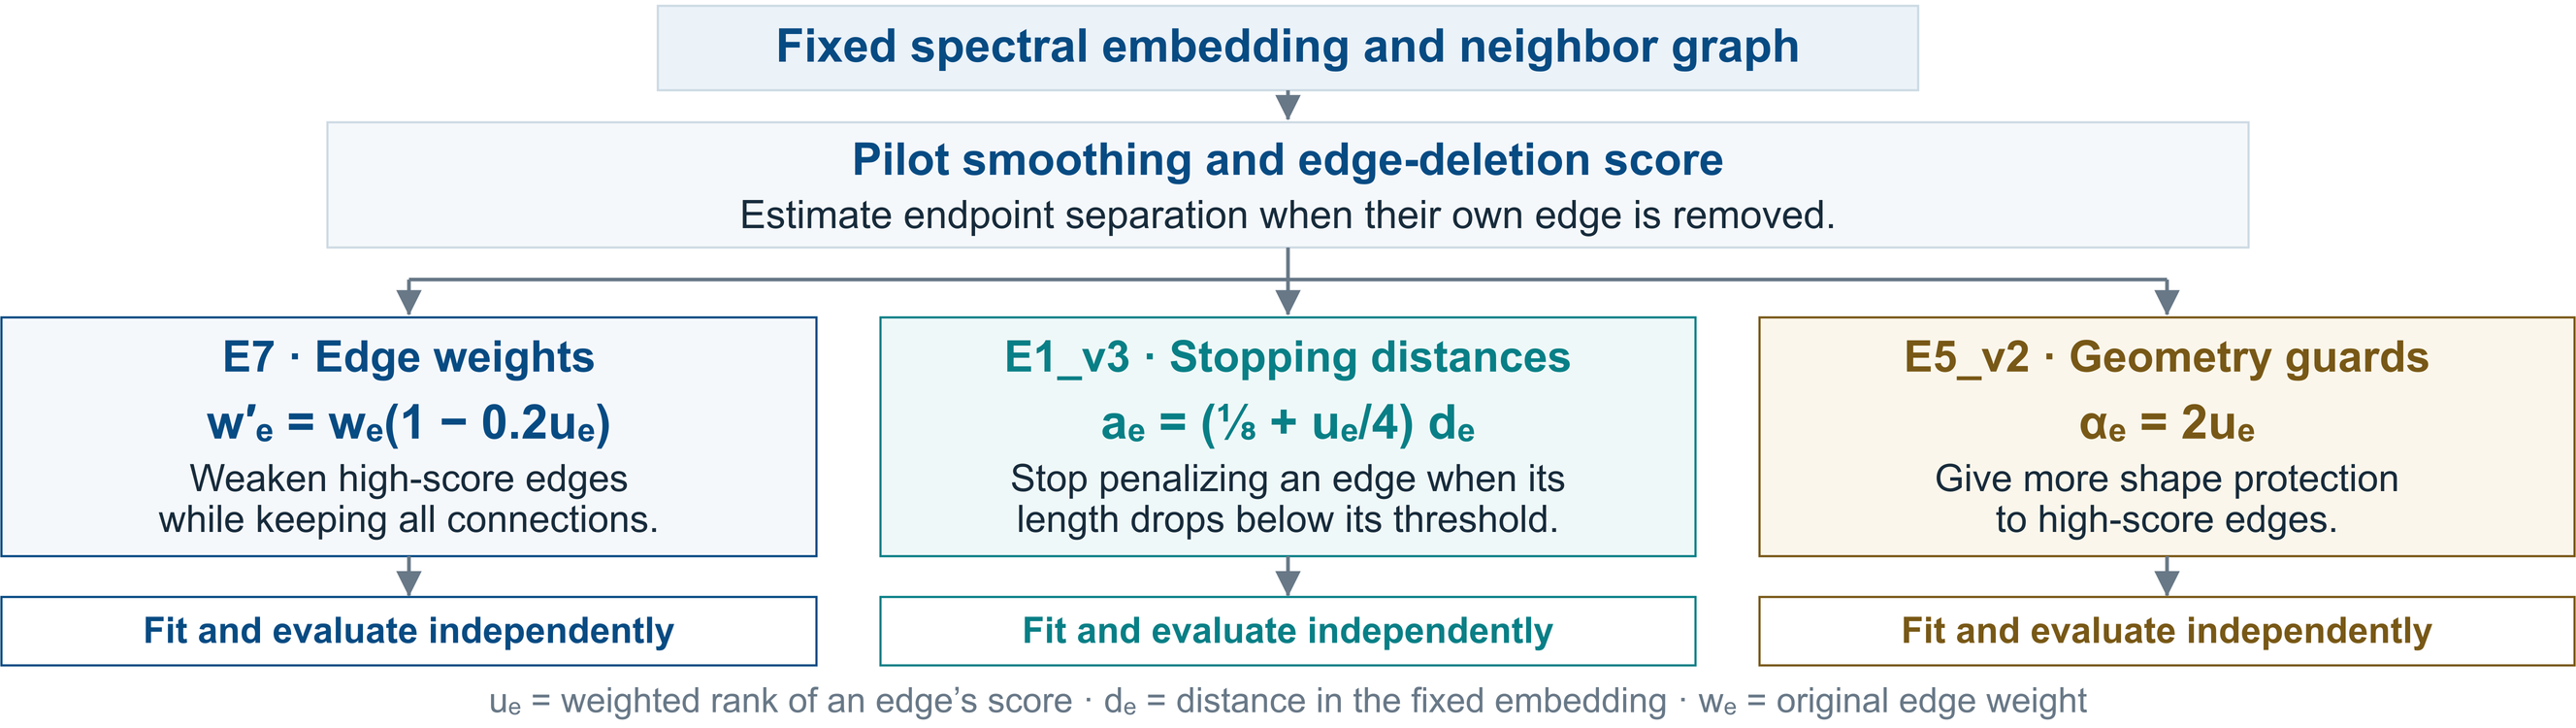
\includegraphics[width=\linewidth]{extension_pipeline_ppt_6_2.png}
\caption{The exact three-branch pipeline from presentation slide 6.2.
The interventions are alternatives and are fitted independently.}
\label{fig:selected_extensions}
\end{figure}

\subsection{Shared evidence and objectives}

Let $F$ denote the frozen anchor after the declared preprocessing, $C$ the
unweighted incidence matrix with each positive undirected edge stored once,
and $w_e$ its weight. Set $L=C^\top\operatorname{diag}(w)C$,
$\tau=1/\operatorname{median}_{d_i>0}d_i$ for weighted node degrees $d_i$,
$M=I+\tau L$ and $Z=M^{-1}F$. For the incidence vector $c_e$ of edge $e$,
\begin{equation}
\ell_e=\tau w_e c_e^\top M^{-1}c_e,
\qquad s_e=\frac{\|c_e^\top Z\|_2^2}{(1-\ell_e)^2}.
\label{eq:edge_score}
\end{equation}
Rank-one inversion gives the exact endpoint discrepancy after deleting one
pilot edge while keeping $\tau,F$ fixed. This adapts the leverage-adjustment
idea discussed by \citet{wang2018alo}; it neither recomputes the spectral
embedding nor estimates the probability that an edge crosses classes.

Write $d_e=\|(CF)_e\|_2$, $r_e(G)=\|(CG)_e\|_2$, and let $u_e$ be the
weighted midrank of $s_e$. Rank masses are $w_e$ for E7/E5\_v2 and $w_ed_e$
for E1\_v3. All three minimize
$\frac12\|G-F\|_F^2+\lambda R(G)$, using
\begin{align}
R_{\rm E7}(G)&=\sum_e w_e(1-0.2u_e)r_e(G),\\
R_{\rm E1}(G)&=\sum_e w_e[r_e(G)-(\tfrac18+\tfrac14u_e)d_e]_+,\\
R_{\rm E5}(G)&=\sum_e w_e\{r_e(G)+2u_e\kappa_e(G)\},\\
\kappa_e(G)&=r_e(G)+\|(C(G-F))_e\|_2-d_e.
\end{align}
Here $[x]_+=\max(x,0)$. E7 weakens high-score edges without deleting support.
E1\_v3 stops penalizing sufficiently short edges; it is not a hard
distance-preservation constraint. E5\_v2 allocates extra triangle-slack
penalty to high-score edges. Weighted ranks preserve fixed allocation budgets.
QSSC uses $R_Q(G)=\sum_e w_er_e(G)$ with the same quadratic fidelity.
The original SSC reference instead uses unsquared row-wise fidelity.

\subsection{Evaluation and qualification}

The eight cohorts are frozen from Appendix~\ref{app:reconstruction}.
Within each cohort, QSSC, the three extensions and their controls share $F,W$
and target relative movement
$\rho=\|G-F\|_F/\|F-\bar F\|_F=0.10$, with $\bar F$ the repeated row mean.
The original SSC reference follows its separately declared fit, without this
movement constraint. Each finite output is evaluated with
50 one-start greedy K-means++ runs. Native initialization generates centers
on each $G$; the common-index panel uses sample indices generated on $F$ and
takes the corresponding rows of each $G$. Labels are used only for evaluation
and post-fit diagnostics after the cohorts and numerical settings are fixed.

Each extension is compared with QSSC and with the same intervention using
the plain score $\|c_e^\top Z\|_2^2$, without deletion correction. Uniform and
shuffled allocations are additional recorded controls. Qualified fits require
relative primal--dual gap $\le10^{-6}$, capacity residual $\le10^{-8}$,
movement uncertainty $e_\rho\le0.005\rho$, and
$|\widehat\rho-\rho|+e_\rho\le0.01\rho$. Aggregate differences use the same
qualified cohort mask for both metrics. They are descriptive conditional means,
not significance claims across independently sampled datasets.

\begin{table}[!htbp]
\centering
\caption{Primary native-panel results corresponding to presentation slide 6.3.
Each cell is mean ACC/NMI (\%) over 50 starts. The SSC reference is separately
fitted and must not be substituted for the historical results in
Table~\ref{tab:reconstruction}. $\dagger$ marks measured but unqualified outputs.}
\label{tab:extension_eight}
\footnotesize
\setlength{\tabcolsep}{2.5pt}
\begin{tabular}{@{}lrrrrrr@{}}
\toprule
Dataset & SC & SSC ref. & QSSC & E7 & E1\_v3 & E5\_v2 \\
\midrule
AR
 & 68.979/84.187 & 57.148/80.588 & 69.131/84.154
 & 69.155/84.079 & 69.150/84.158 & 69.202/84.008 \\
JAFFE
 & 95.305/94.134 & 95.305/94.091 & 95.305/94.136
 & 95.305/94.136 & 95.089/94.055 & 95.089/94.052 \\
ORL
 & 78.325/89.874 & 74.520/89.657 & 78.775/90.000
 & 78.800/90.029 & 78.665/90.372 & 78.445/90.075 \\
UMIST
 & 63.950/81.002 & 70.110/85.234 & 64.348/81.073
 & 64.291/81.131 & 65.521/82.602 & 65.635/82.505 \\
BinAlpha
 & 49.908/60.795 & 32.162/49.862 & 50.644/61.144
 & 50.405/61.182 & 50.438/61.209 & 50.872/61.428 \\
MSRA50
 & 47.117/60.281 & $47.759/61.425^{\dagger}$ & 47.344/61.068
 & 47.310/61.043 & $47.614/60.057^{\dagger}$
 & $47.164/60.449^{\dagger}$ \\
YaleB
 & 45.148/54.367 & 44.249/52.648 & 44.694/53.990
 & 44.664/54.012 & $45.012/53.988^{\dagger}$ & 44.620/53.693 \\
USPS
 & 65.597/80.315 & 66.263/80.856 & 65.621/81.358
 & 65.759/81.414 & 65.901/81.616 & 66.301/81.521 \\
\bottomrule
\end{tabular}
\end{table}

The E1\_v3 MSRA50/YaleB and E5\_v2 MSRA50 outputs are finite and numerically
certified, but reach movements 0.027871/0.070613 and 0.075561, respectively,
instead of the target within the runtime limit. They are excluded from matched
macros. The MSRA50 SSC reference is finite but lacks an optimality certificate;
this is a different reason for its $\dagger$. Per-seed measurements, sample SD
and control records remain in
\path{results/extension_round3/}.

\begin{table}[!htbp]
\centering
\caption{Controlled macro differences, $\Delta$ACC/$\Delta$NMI in pp.
P denotes the corresponding plain-pilot intervention. All rows use
$\rho=0.10$ and pilot-strength multiplier 1. Different partial masks cannot
support a ranking between methods.}
\label{tab:extension_controls}
\small
\setlength{\tabcolsep}{4pt}
\begin{tabular}{@{}lcrrr@{}}
\toprule
Method & Cohorts & Native vs QSSC & Native vs P & Common indices vs P \\
\midrule
E7 & 8/8
 & $-0.022/+0.013$ & $+0.004/-0.001$ & $-0.001/-0.001$ \\
E1\_v3 & 6/8
 & $+0.157/+0.358$ & $-0.123/-0.068$ & $+0.014/+0.009$ \\
E5\_v2 & 7/8
 & $+0.235/+0.204$ & $+0.061/+0.045$ & $+0.004/+0.003$ \\
\bottomrule
\end{tabular}
\end{table}

\paragraph{What the results support.}
E7 is effectively unchanged; E1\_v3's gains against QSSC do not survive its
native plain-pilot control. E5\_v2 has a limited positive signal: on UMIST
it improves over QSSC by 1.287/1.432 pp, while remaining 4.475/2.729 pp below
the original SSC reference. Its extra macro gain nearly vanishes with common
initialization indices. Thus changes in the intervention and rounding must be
separated from benefits specifically due to deletion correction.

The edge score's cross-class AUROC improves only on ORL
($0.838901\to0.839508$) and USPS ($0.752293\to0.752378$), and decreases
on the other six cohorts. E5\_v2 reduces weighted triangle slack to
20.4--40.9\% of QSSC's on its seven qualified cohorts, but reduces both
within-class and between-class variation. It changes the intended geometry
without reliably improving class separation. A plausible limitation is that
deleting one edge cannot expose mutually supporting incorrect neighborhoods
or restore missing within-class connections; this is an explanation consistent
with the results, not a separately established causal finding.
}
